\section{7日目}
\begin{frame}
	\frametitle{なにで書く? \textcircled{1}}
	オープンソースなLua IDEであるZeroBrane Studio\footnote[frame]{\url{http://studio.zerobrane.com}}%
	にはMoonScript用プラグイン\footnote[frame]{\url{https://github.com/pkulchenko/ZeroBranePackage/blob/master/moonscript.lua}}があり、導入することでMoonScriptもバンバン書ける。
\end{frame}

\section{8日目}
\begin{frame}[fragile]
	\frametitle{なにで書く? \textcircled{2}}
	Howl Editor\footnote[frame]{\url{http://howl.io}}はMoonScriptで拡張が書ける! MoonScriptも書ける! 一石二鳥!!

	\begin{columns}	
		\column[t]{.5\hsize}
		\tiny
		\begin{lstlisting}[numbers=none,language=MoonScript]
		import config from howl


		config.hungry_completion = true

		howl.bindings.push {
	editor:
		shift_alt_c: 'editor-toggle-comment'
	ctrl_f: 'open'
	alt_e: 'cursor-word-right'
	alt_w: 'cursor-word-left'
	alt_s: 'save'
	ctrl_w:
		ctrl_w: 'quit'
	r:      'editor-redo'
	u:      'editor-undo'
}

howl.command.vi_on!
	\end{lstlisting}
	\column[t]{.5\hsize}
	\begin{figure}[h]
		\centering
		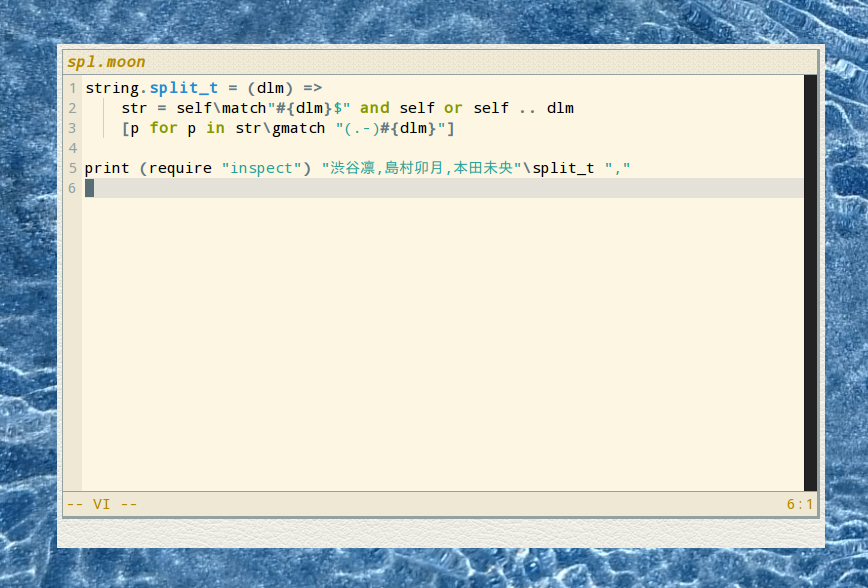
\includegraphics[width=\columnwidth]{img/howl.png}
		\end{figure}
	\end{columns}
\end{frame}
\section{9日目}
\section{10日目}
\section{11日目}
\section{12日目}
